\documentclass[11pt]{article}
\usepackage[review]{acl} % Change review to final for a named course submission.
\usepackage{times}
\usepackage{latexsym}
\usepackage[T1]{fontenc}
\usepackage[utf8]{inputenc}
\usepackage{microtype}
\usepackage{inconsolata}
\usepackage{graphicx}
\usepackage{amsmath}
\usepackage{booktabs}

% Working draft; Methods, Results, and experimental appendices added for feedback.
\title{Belief-State Control for Diplomatic Negotiation with a Lower-Cost Language Model}
% USER EDIT: replace this anonymous line with the actual team information.
% For a named course PDF, also change [review] to [final] in main.tex.
% Keep this file in English / romanized names when compiling with pdfLaTeX.
% Example (uncomment and replace values; do not submit placeholders):
% \author{First Author \and Second Author \\
%   Department, University \\
%   Student IDs: first ID, second ID}
% Actual roles and teammate reproduction are recorded separately in TEAM_RECORD.txt.
\author{Anonymous ACL submission}


\usepackage{capt-of}
% Add a non-floating, full-width teaser to ACL's title block.
\newcommand{\paperteaser}{%
  \begin{minipage}{\textwidth}
  \centering
  \captionsetup{hypcap=false}
  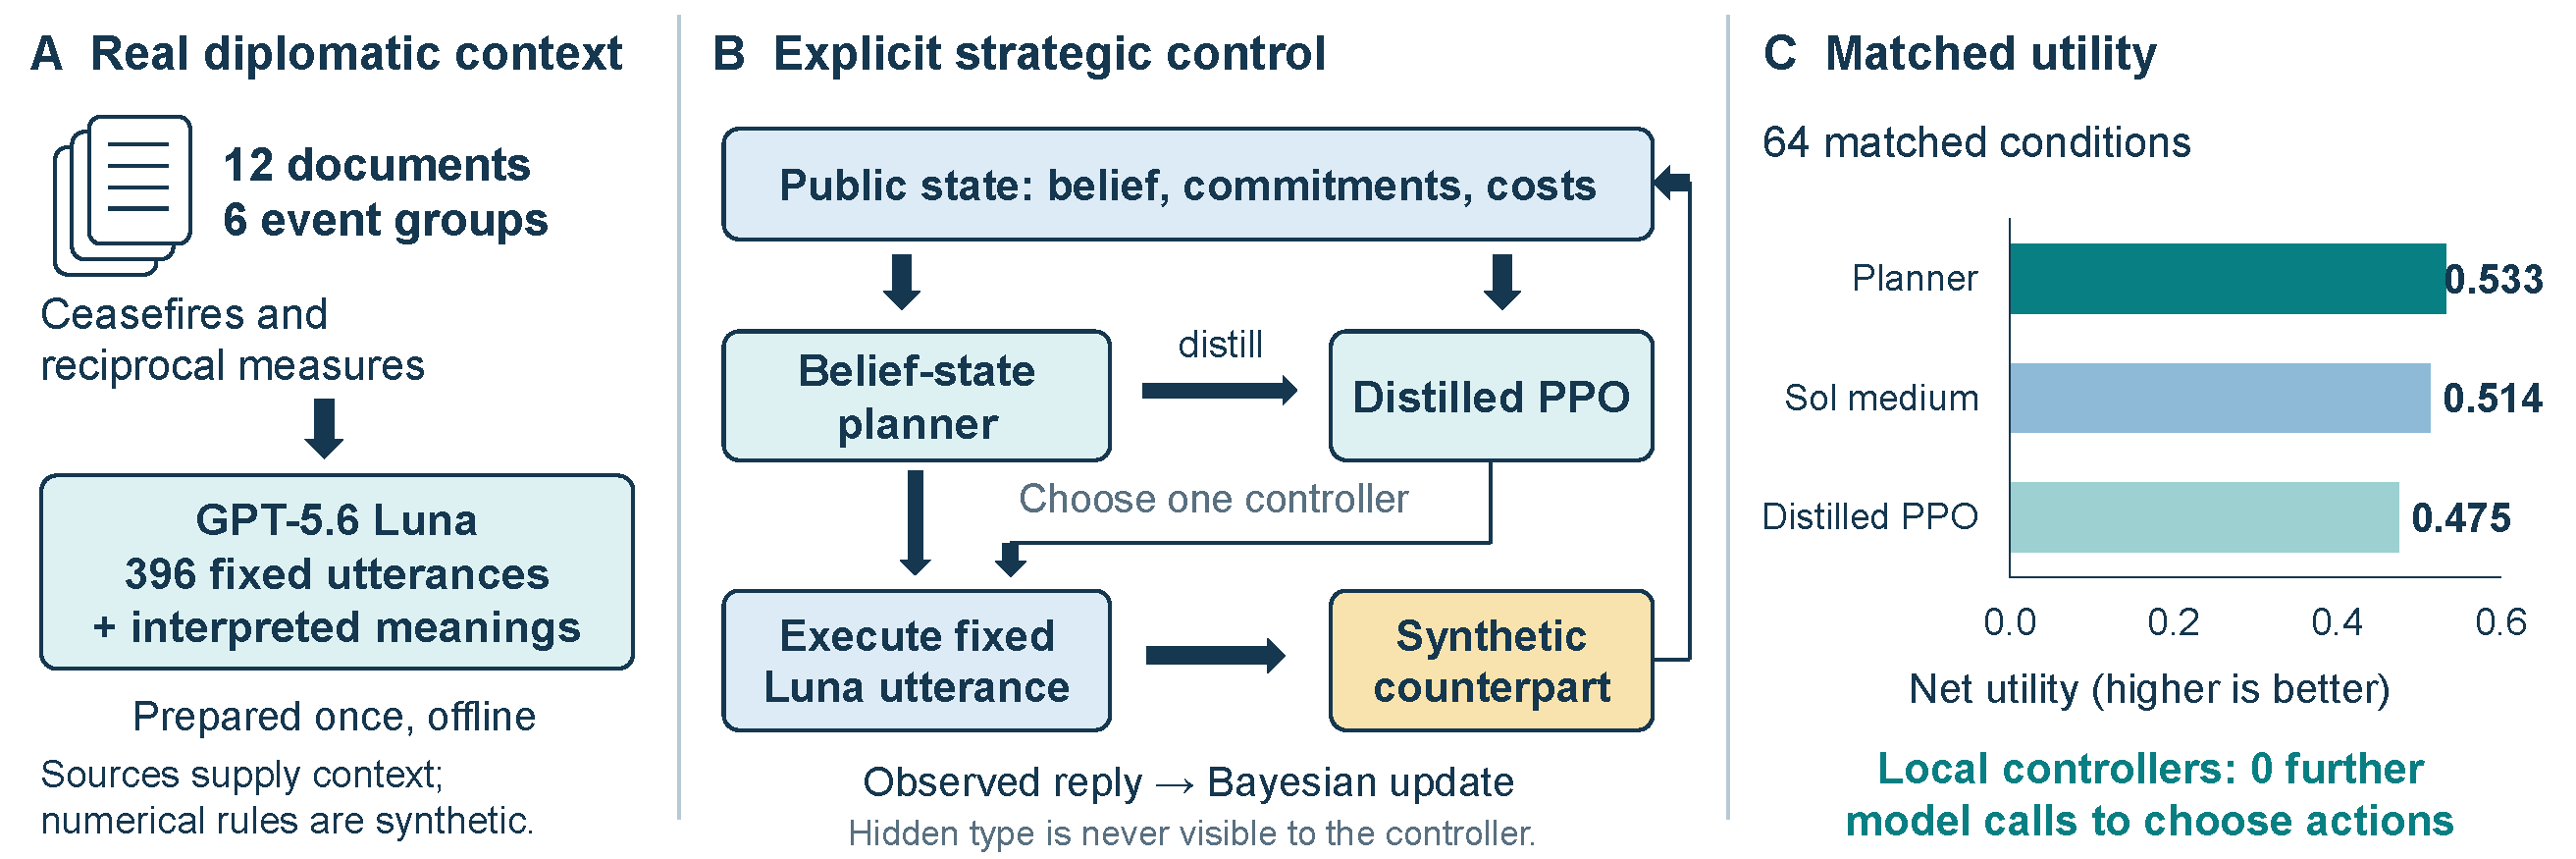
\includegraphics[width=\textwidth]{figures/teaser.pdf}
  \captionof{figure}{Real diplomatic sources ground fixed Luna utterances. A public-belief planner or its distilled PPO policy selects actions under the same language execution. Responses update public beliefs; distillation transfers planner supervision. Zero further model calls refers only to local strategy selection.}
  \label{fig:teaser}
  \end{minipage}\par\vspace{8pt}%
}
\begin{document}
\makeatletter
\let\acloriginalmaketitle\@maketitle
\def\@maketitle{\acloriginalmaketitle\paperteaser}
\makeatother
\maketitle

\begin{abstract}
Can explicit strategic control improve negotiation with a lower-cost language model? We study a simulation grounded in 12 real diplomatic documents, holding GPT-5.6 Luna's generated utterances and their interpretations fixed across controllers. On 64 matched conditions, belief-state planning achieves net utility 0.533, compared with 0.514 for direct action selection by GPT-5.6 Sol with medium reasoning. Planner-distilled PPO reaches 0.475 without further model calls for strategy selection. Separate interventions attribute most of the learned policy's gain to signals and updated beliefs. Dialogue analysis connects these mechanisms to conditional offers and commitment wording. The results identify the benefits of explicit control under declared negotiation rules.
\end{abstract}

\section{Introduction}
Large language model (LLM) agents create opportunities to negotiate on behalf of users \citep{yao2023react,bianchi2024negotiationarena,zhan2024survey}. They must pursue user goals while reasoning about others' interests and incomplete information \citep{gandhi2023strategic,chan2024negotiationtom}. Benchmarks expose strategic decision challenges \citep{abdelnabi2024stakeholders,lin2024decision}. Repeated decisions make inference cost relevant \citep{kapoor2024agents,hakimov2026price}, motivating specialized lower-cost models \citep{belcak2025small}.

Prior work separates strategy from language generation \citep{he-etal-2018-decoupling,deng2024ppdpp}, combines dialogue with planning \citep{fair2022cicero,yu-etal-2023-prompt}, and improves smaller negotiators through reinforcement learning and distillation \citep{hua2026socialrl,tabacof2026negotiate}. We ask: with language held fixed, how does explicit control affect negotiation utility and action-selection cost?

We construct a diplomatic negotiation simulation from 12 real documents across six event groups. The documents provide context and examples of reciprocal conditions; utilities, hidden opponent types, and responses are synthetic. GPT-5.6 Luna (Luna) generates and separately interprets 396 fixed utterances. We compare Random, Heuristic, Bandit, PPO, direct model decisions, an exact public-belief planner, and a policy distilled from that planner (Figure~\ref{fig:teaser}). The planner knows the simulation rules but never observes the hidden type.

On 64 matched conditions, the planner outperforms direct action selection by GPT-5.6 Sol (Sol) with medium reasoning. Distilled PPO improves on base PPO without further strategy-selection model calls. Interventions and dialogue traces distinguish information-seeking questions from incentive-changing signals and test whether actions preserve expressed commitments. Our contribution links negotiation outcomes, strategic computation, and discourse meaning under controlled language conditions.

\section{Related Work}
\paragraph{Negotiation agents.}
Negotiation dialogue research covers bargaining, multi-party interaction, and human assistance \citep{zhan2024survey,lin2024decision}. \citet{lewis-etal-2017-deal} learn from bargaining dialogues and simulated continuations. Recent benchmarks evaluate economic outcomes and mental-state reasoning \citep{bianchi2024negotiationarena,abdelnabi2024stakeholders,chan2024negotiationtom}. CICERO combines dialogue and strategy in the board game Diplomacy \citep{fair2022cicero}; our contexts come from real diplomatic documents.

\paragraph{Strategic control.}
Separating dialogue acts from language supports explicit strategic control \citep{he-etal-2018-decoupling,deng2024ppdpp,liu-etal-2025-dual}. Other methods use tree search, reasoning demonstrations, or diverse user simulation \citep{yu-etal-2023-prompt,gandhi2023strategic,zhang2024trip}. Belief-state dialogue management explicitly models uncertainty \citep{young2013pomdp}. We compare controllers under fixed utterances and interpretations.

\paragraph{Efficient agents.}
Agent evaluation must consider performance and cost \citep{kapoor2024agents,hakimov2026price}. Policy distillation and Expert Iteration transfer expert decisions into learned policies \citep{rusu2016distillation,anthony2017expert}; recent work trains smaller negotiation models \citep{hua2026socialrl,tabacof2026negotiate}. We instead fix language-model weights and train a separate controller, following the motivation for specialized small-model roles \citep{belcak2025small}.

\section{Method}

\paragraph{Data and task.}

We use 12 document contexts from six diplomatic event groups, including CMFA PressCon \citep{mochtak2021corpus} and Security Council discourse. Training covers the Korean Peninsula, South Sudan, and Kashmir (six contexts); development uses Gaza (two); testing uses Syria and Iran (four). Passages about ceasefires, reciprocal measures, and commitments guide synthetic bilateral negotiations. One party offers to maintain its measure for $x\in\{1,2,3\}$ weeks if the counterpart maintains its measure for $y\in\{1,2\}$ weeks. Durations, payoffs, types, and responses are researcher-defined.

For example, a peninsula briefing links suspending nuclear and missile activities to suspending military exercises. These reciprocal measures become the parties' actions. Documents supply the issues and commitment language; synthetic durations and costs determine acceptance.

\paragraph{State, actions, and reward.}

The agent has at most five decisions and cannot observe the counterpart's type, $\tau\in\{S,H\}$. It observes the offer, acceptance, commitments, costs, and belief $b_t=P(\tau=H)$. Eleven actions cover ambiguity, signaling, a private question, six conditional offers, ratification, and withdrawal. Questions provide noisy type cues; offer responses also reveal information. Ratification requires observed acceptance and own utility at least as high as the outside option.

Specifically, an agreement gives $u_A=0.5y-0.18x$, and the counterpart accepts when $u_B=0.35x-c_\tau y+\delta z\geq0$, where $z$ records a signal and $c_\tau$ determines the cost of reciprocal measures. A signal therefore changes an incentive; a question changes information. For response likelihoods $L_H$ and $L_S$, the public belief becomes
\begin{equation}
 b_{t+1}=\frac{b_tL_H}{b_tL_H+(1-b_t)L_S}.
\end{equation}
Equal response likelihoods leave the belief unchanged. Step rewards are
\begin{equation}
 r_t=d_tu_{\mathrm{end}}-0.01-c^{\mathrm{act}}_t-0.005e_{t+1}^2,
\end{equation}
where $d_t$ marks termination, $e$ counts rejected offers, and $c^{\mathrm{act}}_t$ sums question, signal, rejection, reversal, and invalid-action charges. Terminal utility is $u_A$ at agreement or 0.12 at withdrawal or expiration, paid once. We report $\sum_t r_t$. Appendix~\ref{app:environment} gives all costs and transition rules.

\paragraph{Shared language execution.}

GPT-5.6 Luna generates three styles per context--action pair, yielding 396 utterances. A separate Luna call interprets their function, reciprocal terms, and stated cost. These meanings determine transitions; interpretation mismatches are retained. All controllers share these utterances and templated counterpart replies, separating action selection from language realization.

\paragraph{Strategic controllers.}

We compare Random, a development-selected signal-first Heuristic, an immediate-reward Bandit, and PPO \citep{schulman2017ppo}. An exact belief-state planner maximizes expected net utility under the declared rules without seeing the true type. We distill its action values from training contexts and configurations, then refine the policy with PPO. Direct Luna (reasoning \texttt{none}) and Sol (\texttt{none}/\texttt{medium}) receive the public state and numerical rules.

The planner solves response branches by backward recursion. Following policy distillation and expert-guided learning \citep{rusu2016distillation,anthony2017expert}, we train on 43,440 public states from planner and exploratory trajectories. After 2,400 supervised updates, PPO refines the network. Deployment selects the highest-scoring action from 31 public features.

Planner values $Q_T(s,a)$ define the teacher distribution $p_T(a\mid s)\propto\exp(Q_T(s,a)/0.03)$. The supervised loss is
\begin{equation}
\begin{aligned}
\mathcal{L}={}&-\sum_a p_T(a\mid s)\log\pi_\theta(a\mid s)\\
&+\tfrac12\bigl(V_\theta(s)-\max_a Q_T(s,a)\bigr)^2.
\end{aligned}
\end{equation}
Policy targets preserve action preferences; value targets estimate return. PPO updates both using interaction rewards.

\section{Experimental Setup}

Initial evaluation crosses four contexts, 64 configurations, and three styles. Matched evaluation uses the first 16 configurations and one style (64 conditions); follow-up uses 64 new configurations and three styles. We take expectations over types and question responses, then average within and across event groups. Bandit and base PPO receive 102,400 steps per seed; distillation adds teacher supervision. Learned results average three seeds, using final checkpoints and development-selected methods. Appendices~\ref{app:training} and~\ref{app:diagnostics} give settings and diagnostics.

Every matched controller encounters the same context, numerical rules, utterances, and response-branch probabilities. We enumerate nonzero branches rather than relying on a single sampled counterpart, so differences reflect action choices under the shared environment.

\section{Results}

\begin{table}[t]
\centering\small
\setlength{\tabcolsep}{3pt}
\begin{tabular}{lrrr}
\toprule
Controller & Utility & Agree. & Calls \\
\midrule
\multicolumn{4}{l}{\textit{A. Initial: 256 conditions, three styles}} \\
Random & -0.146 $\pm$ 0.001 & 11.0 & 0 \\
Bandit & 0.118 $\pm$ 0.001 & 23.8 & 0 \\
Heuristic & 0.419 & 94.8 & 0 \\
PPO & 0.358 $\pm$ 0.018 & 73.0 & 0 \\
Planner & 0.488 & 93.3 & 0 \\
\midrule
\multicolumn{4}{l}{\textit{B. Matched: 64 conditions, one style}} \\
Luna none & -0.368 & 24.3 & 3.949 \\
Sol none & -0.367 & 26.3 & 4.773 \\
Sol medium & 0.514 & 100.0 & 3.429 \\
Heuristic & 0.470 & 100.0 & 0 \\
PPO & 0.378 $\pm$ 0.012 & 81.9 & 0 \\
Distilled PPO & 0.475 $\pm$ 0.016 & 98.3 & 0 \\
Planner & 0.533 & 100.0 & 0 \\
\bottomrule
\end{tabular}
\caption{Policy comparison with fixed Luna utterances. Agreement is a percentage; calls are per negotiation for strategy selection. $\pm$: three-seed SD (evaluation seeds for Random). Panels use different conditions.}
\label{tab:policies}
\end{table}

\begin{figure}[t]
\centering
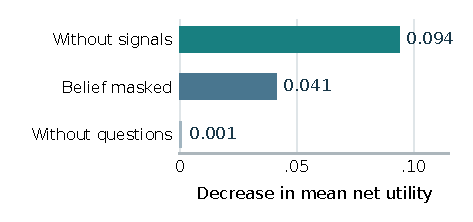
\includegraphics[width=\columnwidth]{figures/intervention_losses.pdf}
\caption{Evaluation-time interventions on distilled PPO. Losses are differences in three-seed mean utility on the follow-up conditions. Full values and seed variation appear in Table~\ref{tab:interventions}.}
\label{fig:interventions}
\end{figure}

Initially, PPO outperforms Random and Bandit but falls below the heuristic (Table~\ref{tab:policies}). In the matched comparison, the planner reaches 0.533 utility versus 0.514 for Sol medium. Distilled PPO reaches 0.475 versus 0.378 for base PPO and 0.470 for the heuristic. Sol none remains near Luna none: direct-model performance depends strongly on reasoning settings.

Local controllers require no language model calls for action selection. Sol medium uses an expected 3.429 calls per negotiation, corresponding to 4,184.8 tokens and \$0.02363 at the recorded request costs. These figures count logical requests even when experimental caching avoids a repeated call. These strategy-selection figures exclude shared utterance construction, interpretation, and offline training.

Distilled PPO gains 0.097 utility over base PPO and remains 0.039 below Sol medium. Offline planner supervision thus offers a deployment trade-off, reducing repeated model-based decision costs while recovering part of the stronger controller's performance.

On the follow-up configurations, distilled PPO achieves 0.468 utility, compared with 0.364 for base PPO and 0.445 for the heuristic (Figure~\ref{fig:interventions}). Blocking signals reduces utility by 0.094; replacing the posterior feature with the prior reduces it by 0.041. Blocking questions reduces it by only 0.001. These are evaluation-time interventions without retraining. The learned policy benefits mainly from signals and updated beliefs in this setting. Updated beliefs can come from offer responses as well as questions. The planner's no-question comparison yields a larger utility loss of 0.008.

\paragraph{Discourse analysis.}

\begin{figure}[t]
\centering
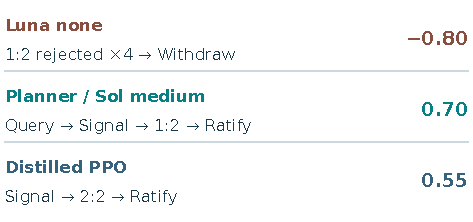
\includegraphics[width=\columnwidth]{figures/discourse_paths.pdf}
\caption{Selected paths under the same Iran-context condition and soft counterpart. Terms $x$:$y$ denote own and reciprocal durations. Values are episode net utility; the learned path uses seed 17.}
\label{fig:discourse}
\end{figure}

Matched Iran-context traces illustrate this distinction (Figure~\ref{fig:discourse}). Luna none repeats a rejected 1:2 offer four times and withdraws, yielding $-0.80$. The planner and Sol medium ask a private question, send a signal, and obtain acceptance of that same offer, yielding 0.70. The question changes the belief from 0.65 to 0; the signal raises the soft counterpart's acceptance utility from $-0.05$ to 0.05. The learned controller instead signals and offers 2:2, yielding 0.55. Wording also matters: in a Syria-context pair, explicit withdrawal terminates the episode, while conditional withdrawal is interpreted as invalid and incurs repeated costs. Appendix~\ref{app:discourse} examines these paths and distinguishes expressed readiness to ratify from ratification itself.

Both types reject the unsignaled 1:2 demand, so repetition provides no new information. A question resolves uncertainty; the subsequent signal makes the demand acceptable. The learned policy instead concedes more. Successful agreement therefore does not establish that it reproduces the planner's information-gathering strategy.


\section{Discussion}
Our results support assigning explicit strategic decisions to a separate controller when the negotiation rules can be specified. The planner uses beliefs, action costs, and future consequences to improve decisions under the same language conditions. Distillation transfers part of this behavior to a policy that acts without search or further language model calls. Its improvement over base PPO shows the value of planner supervision in this setting. Its remaining gap to Sol medium and small advantage over the heuristic distinguish exact planning from learned control.

The interventions suggest that asking more questions is not the main source of the learned policy's improvement. Signals change acceptance incentives, while responses to offers can update beliefs without a separate question. Useful information therefore depends on what the agent can subsequently do with it and what obtaining it costs. Discourse analysis adds a complementary requirement: the chosen action must be expressed with the intended conditions and commitment strength. A conditional threat to withdraw and an actual withdrawal can lead to different transitions. Strategic evaluation should therefore connect utility, information use, and the meaning of the resulting utterance.

\section{Conclusion}
We studied strategic control for a lower-cost language model in a diplomatic negotiation simulation grounded in real documents. With utterances held fixed, belief-state planning achieved the highest utility in the matched comparison, and planner-distilled PPO improved on base PPO without further model calls for action selection. Interventions linked the learned policy's gains mainly to signals and updated beliefs. Dialogue traces further showed how information use and commitment wording shape negotiation paths. These findings identify explicit strategic control as a useful component of negotiation systems and show how controlled comparisons can explain its benefits.


\section*{Limitations}
Payoffs and dialogues are synthetic despite real-document grounding. Four test contexts cover only two event groups. Fixed utterances limit online-dialogue claims; all 44 matched style-0 meanings equal canonical templates, so utility cannot establish a generation advantage. Shared-model interpretation lacks human validation and misclassifies some commitments. Models also assisted drafting and a visual concept.

Known rules and teacher computation advantage planning and distillation over model-free learning. Model mismatch is untested; reasoning settings do not isolate model size. Three seeds and one cached response per state omit historical and output uncertainty. Reported costs exclude language preparation, teacher supervision, training, and local computation. Appendices~\ref{app:environment}--\ref{app:discourse} give details.


% All pre-reference content, including Limitations, stays within four pages.
% References follow the text naturally; no forced page or column break.
\bibliography{references}

\clearpage
\appendix
\section{Implementation and Reproducibility}
\label{app:environment}
\paragraph{Environment.}
The soft-type cost is $c_S=0.2$. A first question yields a type cue with accuracy $q$; later questions give no new cue. Each turn costs 0.01, each question $c_q$, and each rejection $c_r$, plus the escalation cost in the main text. Signals incur their interpreted expenditure (intended 0.06), set $z=1$, and do not stack. Reducing an offered duration below the recorded commitment costs 0.08. Ambiguity makes the next offer provisional without erasing prior commitments. Invalid interpretations or ratifications cost 0.10. Ratification requires observed acceptance and $u_A\geq0.12$; withdrawal or expiration pays 0.12 before costs.

We draw 96 training, 32 development, 64 initial test, and 64 new follow-up configurations over priors, question reliability/cost, rejection cost, signal effect, and hard-type cost. Exact grids are released. The 31 public features exclude source identity and hidden type. All 17 mismatches among 396 intended/interpreted action pairs remain; these are automatic checks, not human labels.

\paragraph{Training and aggregation.}
\label{app:training}
PPO uses two 64-unit layers, learning rate $3\times10^{-4}$, discount .95, entropy .01, rollout 256, batch 64, and ten epochs. Bandit exploration is .2. Both use seeds 17, 29, and 43. Distillation uses Adam at .001, batches of 256, value-loss weight .5, and gradient clipping .5; 35\% random exploration augments teacher trajectories. Teacher computation is additional to PPO interaction. Evaluation averages styles and configurations within event groups, then weights groups equally. SD is across seeds, not historical events. Follow-up interventions appear in Table~\ref{tab:interventions}. Single-seed training ablations yield .346/.327 for discount .8/.99, .366/.392 for entropy 0/.1, and .377/.371 without rejection/reversal costs.

\paragraph{Released detail.}
Source sentences and provenance are in \texttt{study\_results/contexts.json}. The repository includes traces, checkpoints, reproduction commands, and the unabridged supplement in \texttt{paper/supplementary\_appendix\_full.tex}.

\section{Six Discourse Cases}
\label{app:discourse}
These are synthetic, source-grounded episodes, not historical dialogues. Cases 1--4 share Iran context \texttt{ir1} (UNSC S/2020/644, 30 June 2020), condition 0, style 0, and the soft-type evaluation branch. Cases 5--6 share Syria context \texttt{sy1} (CMFA briefing, 1 March 2016), condition 25, and the hard-type branch. Hidden types are not controller inputs.

\paragraph{1. Luna none.}
``We will suspend the specified sanctions for 1 week, conditional upon your suspension of the specified nuclear activities for 2 weeks'' is rejected and repeated three times before withdrawal. Both types reject this unsignaled offer, so belief stays .65. Repetition adds costs without information; net utility is $-.80$.

\paragraph{2. Planner.}
``Privately, we ask whether you require a larger reciprocal concession'' elicits a soft response, reducing belief to zero. A signal then changes counterpart utility for the 1:2 offer from $-.05$ to .05. Question, signal, offer, and ratification yield .70: the question supplies information; the signal changes incentives.

\paragraph{3. Sol medium.}
Sol follows the same path and shared utterances, also yielding .70. Its final utterance starts ``We reaffirm our readiness to ratify the currently accepted agreement''. The interpreter records ratification, although readiness does not itself perform that act. This is not independent language generation.

\paragraph{4. Distilled PPO, seed 17.}
The policy signals and offers ``We will suspend the specified sanctions for two weeks, provided that you suspend the specified nuclear activities for the same period''. Acceptance reveals the soft type; ratification follows. Utility is .55. It avoids the question but makes a larger concession. The same readiness-to-ratify mismatch applies.

\paragraph{5. Explicit withdrawal.}
After a signal and rejected 2:2 offer, the heuristic says ``We hereby withdraw from these negotiations, without proposing or ratifying any agreement''. The episode ends at $-.14$. Rejection reveals infeasibility; the signal is wasted because its configured effect is zero.

\paragraph{6. Conditional withdrawal.}
With another style, the same policy instead says ``If these negotiations cannot advance without compromising our principles, we will withdraw without proposing or ratifying any agreement.'' The interpreter treats this conditional threat as invalid. Three attempts lead to expiration and $-.47$: three invalid charges and two additional turns and escalation charges explain the .33 loss.

\clearpage
\section{Learning, Transitions, and Rule Sensitivity}
\label{app:diagnostics}

\begin{figure*}[t]
\centering
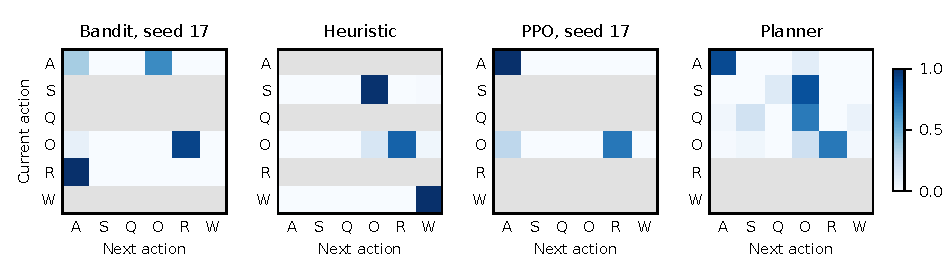
\includegraphics[width=\textwidth]{figures/assignment_transitions.pdf}
\caption{Within-episode action transitions in the initial test evaluation. A: ambiguity; S: signal; Q: question; O: any offer; R: ratify; W: withdraw. We merge six offer actions, then normalize each count row. Grey rows have no outgoing observations. All panels use the same scale.}
\label{fig:course_transitions}
\end{figure*}

\paragraph{Transition counts and interpretation.}
Figure~\ref{fig:course_transitions} summarizes saved action sequences, without connecting different episodes. Original eleven-action counts, weighted counts, and row probabilities are released in \texttt{transition\_matrices.json}; the figure's grouped counts accompany the paper. Counts describe enumerated response paths, not independent historical events or their population frequencies. The illustrative learned panels use seed 17.

Base PPO has 2,260 ambiguity-to-ambiguity transitions and 1,528 transitions from a 3:2 offer to ratification. The Bandit has 312 ambiguity repetitions and 672 transitions from 2:1 to ratification. The heuristic frequently moves from a signal to 2:2 (1,224 transitions); the planner often moves from a signal to 1:2 (836). These patterns connect the aggregate results to different strategic paths. In the implemented rules, ambiguity alone changes commitment status, not the counterpart's information response. Repeated ambiguity can therefore use opportunities without resolving uncertainty. The signal-to-offer pattern instead changes acceptance incentives before proposing terms. Frequencies summarize behavior; the matched cases in Appendix~\ref{app:discourse} provide the actual utterances and consequences.

\begin{figure*}[t]
\centering
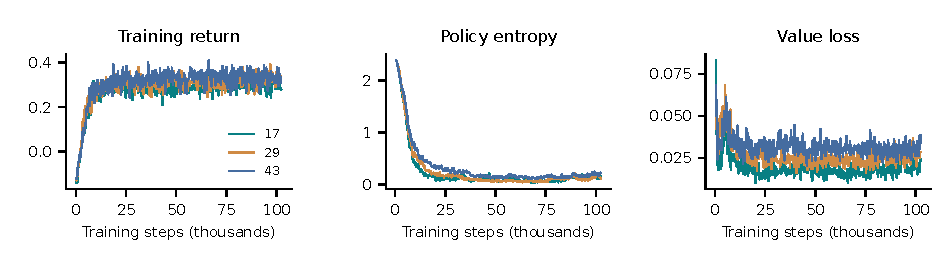
\includegraphics[width=\textwidth]{figures/assignment_learning.pdf}
\caption{Base PPO training diagnostics for seeds 17, 29, and 43. Return is the training logger's rolling episode mean. Entropy is the negative of the logged entropy loss; value loss is shown without additional smoothing. These are training diagnostics, not held-out performance.}
\label{fig:course_learning}
\end{figure*}

\paragraph{Learning stability.}
Training return rises from approximately $-0.14$ to $-0.12$ in the first logged episodes to 0.278, 0.339, and 0.308 at the final checkpoints (Figure~\ref{fig:course_learning}). Policy entropy falls from about 2.40 to 0.152, 0.125, and 0.228. Final value losses are 0.025, 0.028, and 0.039. The policy becomes more concentrated, but low entropy does not establish good negotiation: base PPO asks no questions and sends no signals on the initial test, and remains below the heuristic. Its test utility is $0.358\pm0.018$ across seeds. This motivates adding planner supervision rather than interpreting falling loss as sufficient evidence of success.

\begin{table}[t]
\centering\small
\begin{tabular}{lrrr}
\toprule
Changed rule & Planner & Questions & PPO \\
\midrule
$q=0.50$ & 0.527 & 0.00 & 0.410 \\
$q=0.70$ & 0.528 & 0.00 & 0.410 \\
$q=0.90$ & 0.532 & 1.00 & 0.410 \\
$q=1.00$ & 0.555 & 1.00 & 0.410 \\
$\delta=0.00$ & 0.486 & 1.00 & 0.410 \\
$\delta=0.10$ & 0.532 & 1.00 & 0.410 \\
$\delta=0.25$ & 0.596 & 1.00 & 0.410 \\
\bottomrule
\end{tabular}

\caption{One-factor evaluation-only rule shifts. Planner and PPO columns report utility; Questions is the planner's expected question count. PPO averages three frozen seeds. Other parameters are fixed to the reference configuration.}
\label{tab:course_sensitivity}
\end{table}

\paragraph{Information and rule sensitivity.}
Table~\ref{tab:course_sensitivity} separates question reliability from signal strength. The planner asks no question at reliability 0.5 or 0.7 and asks one at 0.9 or 1.0. Higher reliability becomes useful when it changes the preferred path enough to justify the question cost. Increasing the signal effect from 0 to 0.25 raises planner utility from 0.486 to 0.596. Base PPO stays at mean utility 0.410 across these shifts because it uses neither action in these evaluations. The frozen-policy design tests behavior under changed rules; it does not estimate what retraining would learn. Additional hard-type, rejection-cost, and question-cost sweeps are preserved in \texttt{sensitivity\_metrics.json}.

\begin{table*}[t]
\centering\small
\setlength{\tabcolsep}{3.5pt}
\begin{tabular}{lrrrrrrrrr}
\toprule
Policy & Own & Other & Cost & Break & Turns & Max $e$ & Mean $e$ & Reverse & Viol. \\
\midrule
Random & 0.147 & 0.040 & 0.292 & 0.890 & 4.288 & 0.856 & 0.547 & 0.437 & 0.000 \\
Bandit & 0.140 & 0.082 & 0.022 & 0.762 & 1.773 & 0.030 & 0.017 & 0.000 & 0.000 \\
Heuristic & 0.531 & 0.260 & 0.112 & 0.052 & 3.148 & 0.160 & 0.119 & 0.000 & 0.000 \\
PPO & 0.413 & 0.278 & 0.055 & 0.270 & 2.459 & 0.264 & 0.263 & 0.000 & 0.000 \\
Planner & 0.570 & 0.176 & 0.082 & 0.067 & 3.030 & 0.211 & 0.183 & 0.000 & 0.000 \\
\bottomrule
\end{tabular}

\caption{Additional initial-test metrics, averaged with the same event-group weighting as Table~\ref{tab:policies}A. Own and Other are pre-cost utilities averaged over all outcomes. Break is the breakdown rate, Reverse counts commitment reversals, and Viol. counts bilateral-acceptance violations. Escalation $e$ is a designed rejection index.}
\label{tab:course_metrics}
\end{table*}

\paragraph{Outcome quality and failure.}
Table~\ref{tab:course_metrics} reports both parties' utilities, costs, breakdowns, length, escalation, reversals, and violations. The planner's higher own net utility does not imply higher counterpart utility. No reported terminal agreement violates numerical acceptance conditions. The initial evaluation has a weighted infeasible fraction of 4.7\% under canonical offer and signal options, so withdrawal is not automatically a policy error. Initial discount, entropy, and reward-term training interventions are reported in Appendix~\ref{app:training}; their single-seed status is explicit.

\end{document}
